\documentclass[../presentation.tex]{subfiles} % Parent file
\graphicspath{{\subfix{../images/}}} % Images path

\begin{document}

\section{Conclusion}

\begin{frame}
	\begin{cbox}
		{\fontsize{20pt}{7.2}\selectfont Conclusion}
	\end{cbox}
\end{frame}

\begin{frame}
    
    \frametitle{Conclusion}

		\begin{minipage}{0.49\textwidth}
			\begin{figure}
				\centering
				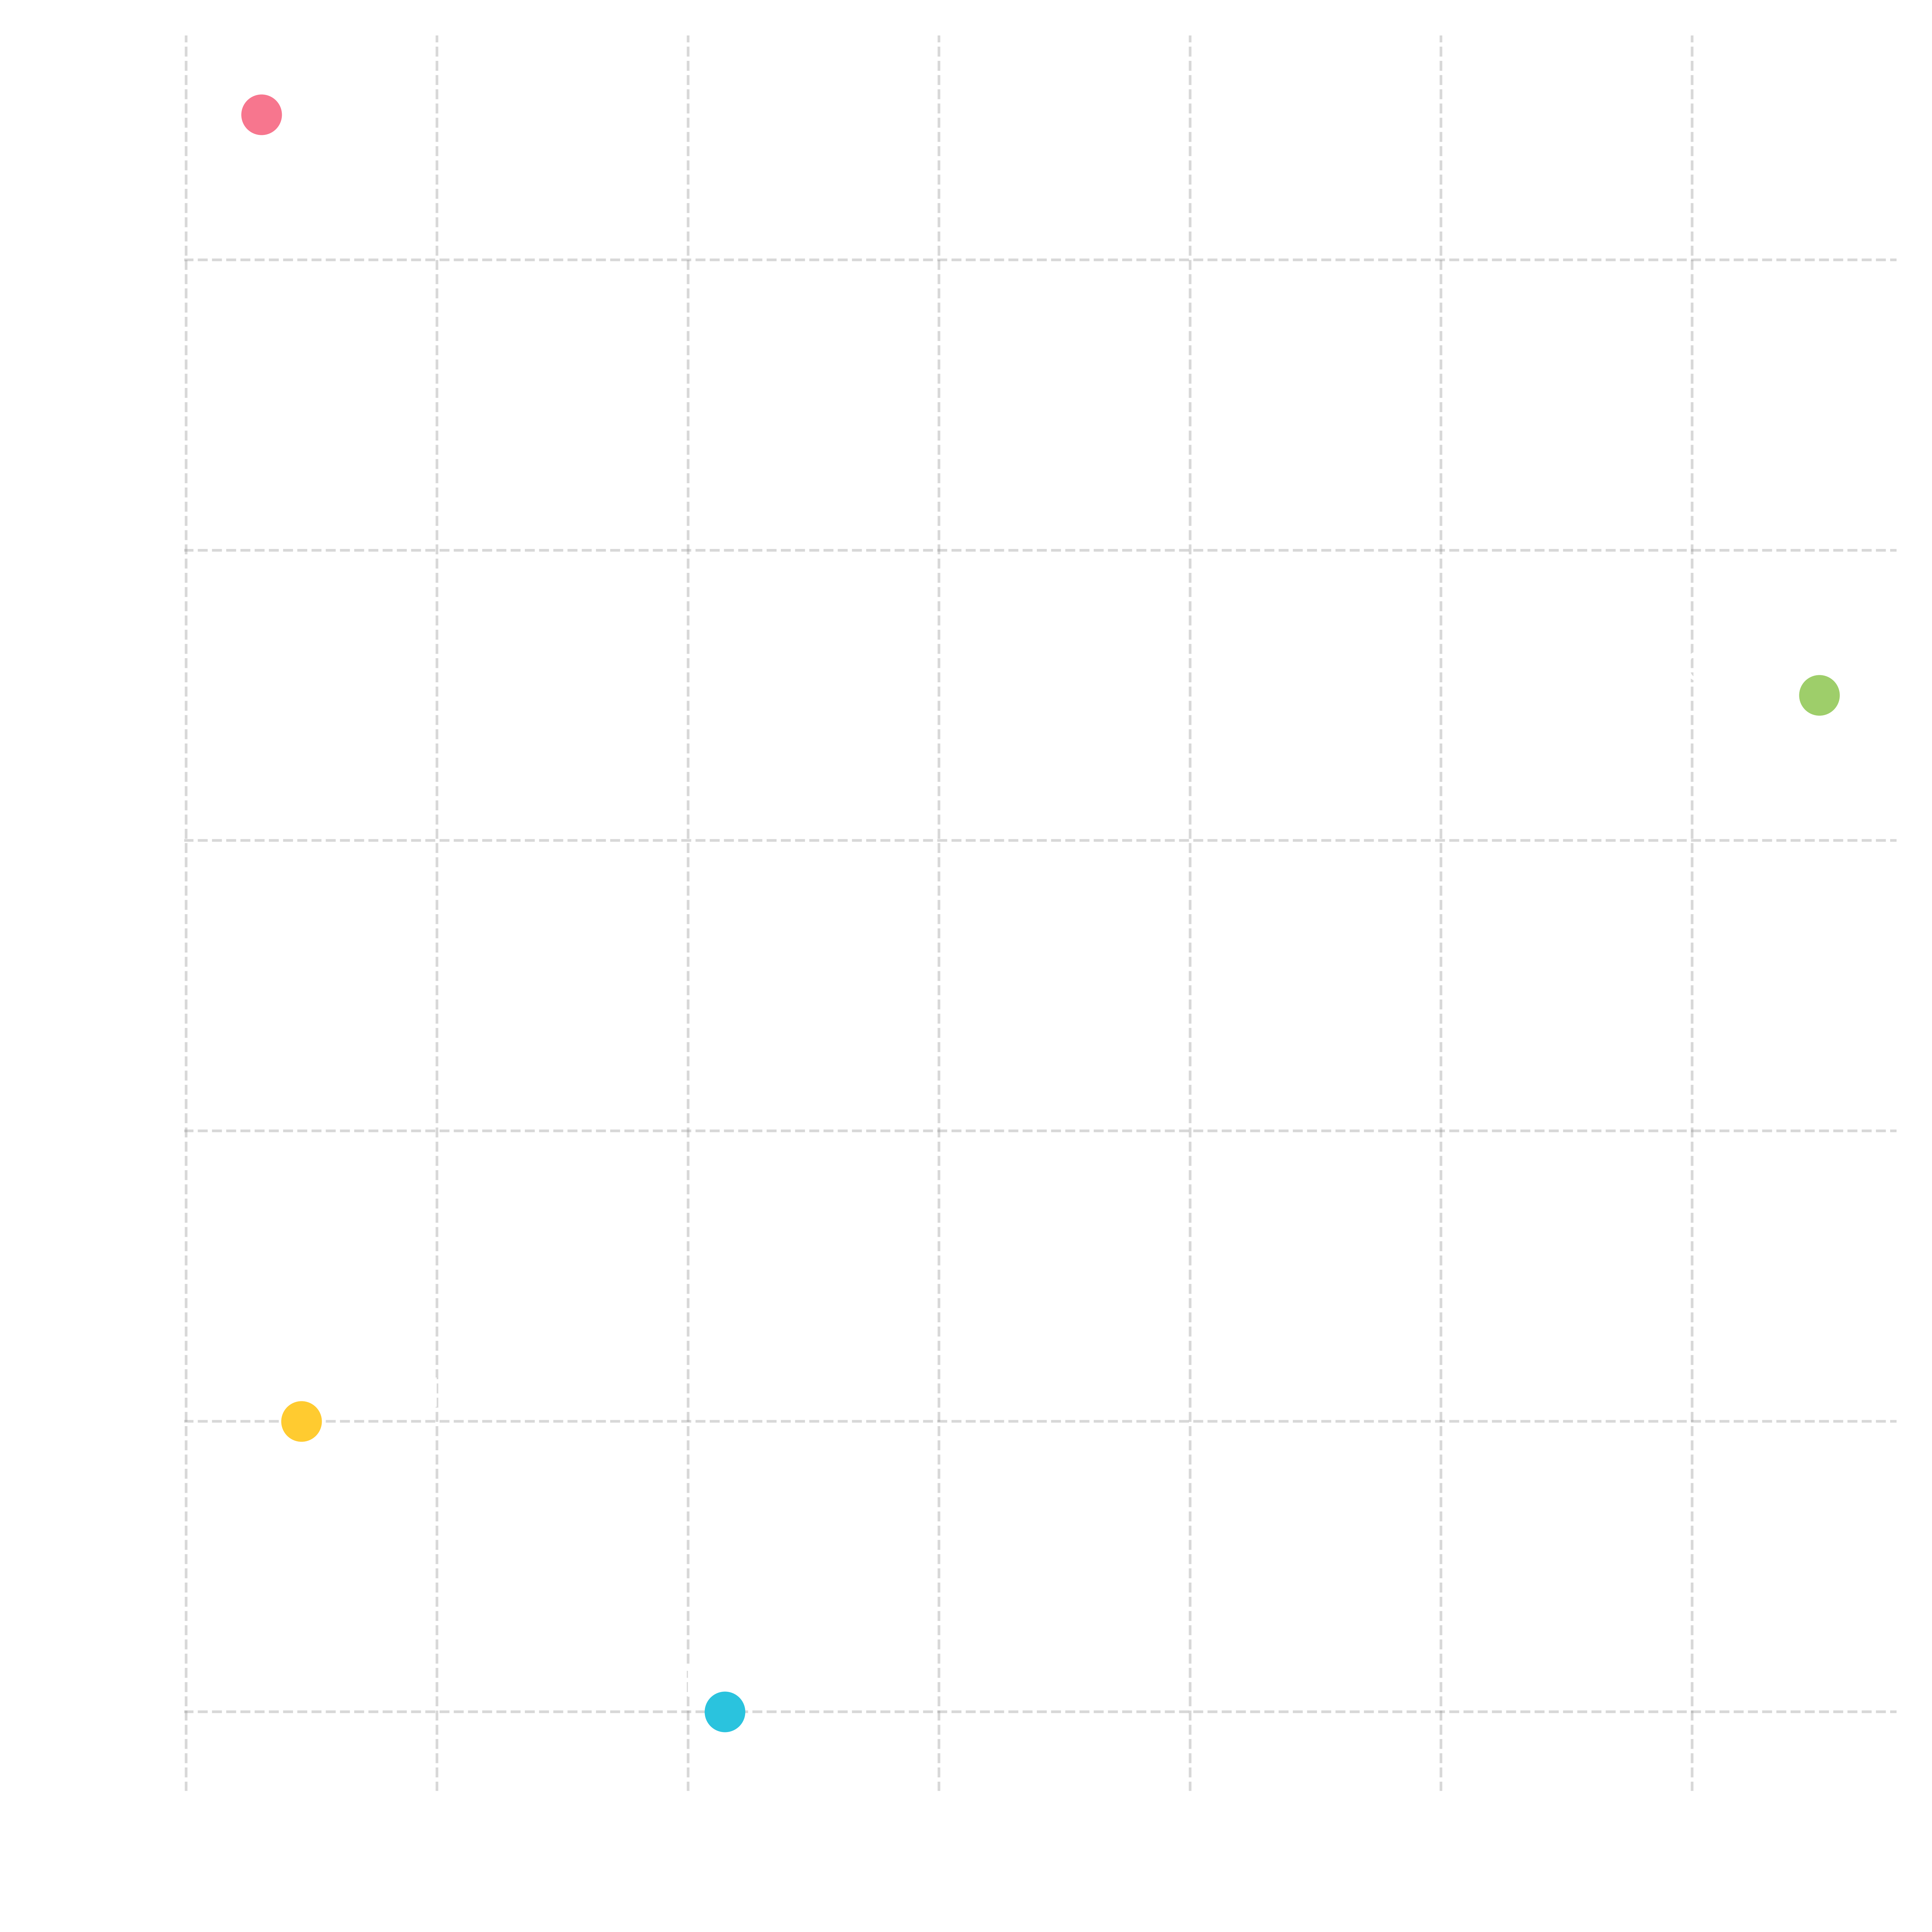
\includegraphics[width=\textwidth]{params_vs_accuracy.png}
			\end{figure}
		\end{minipage}
			\hfill
		\begin{minipage}{0.49\textwidth}
			\begin{figure}
				\centering
				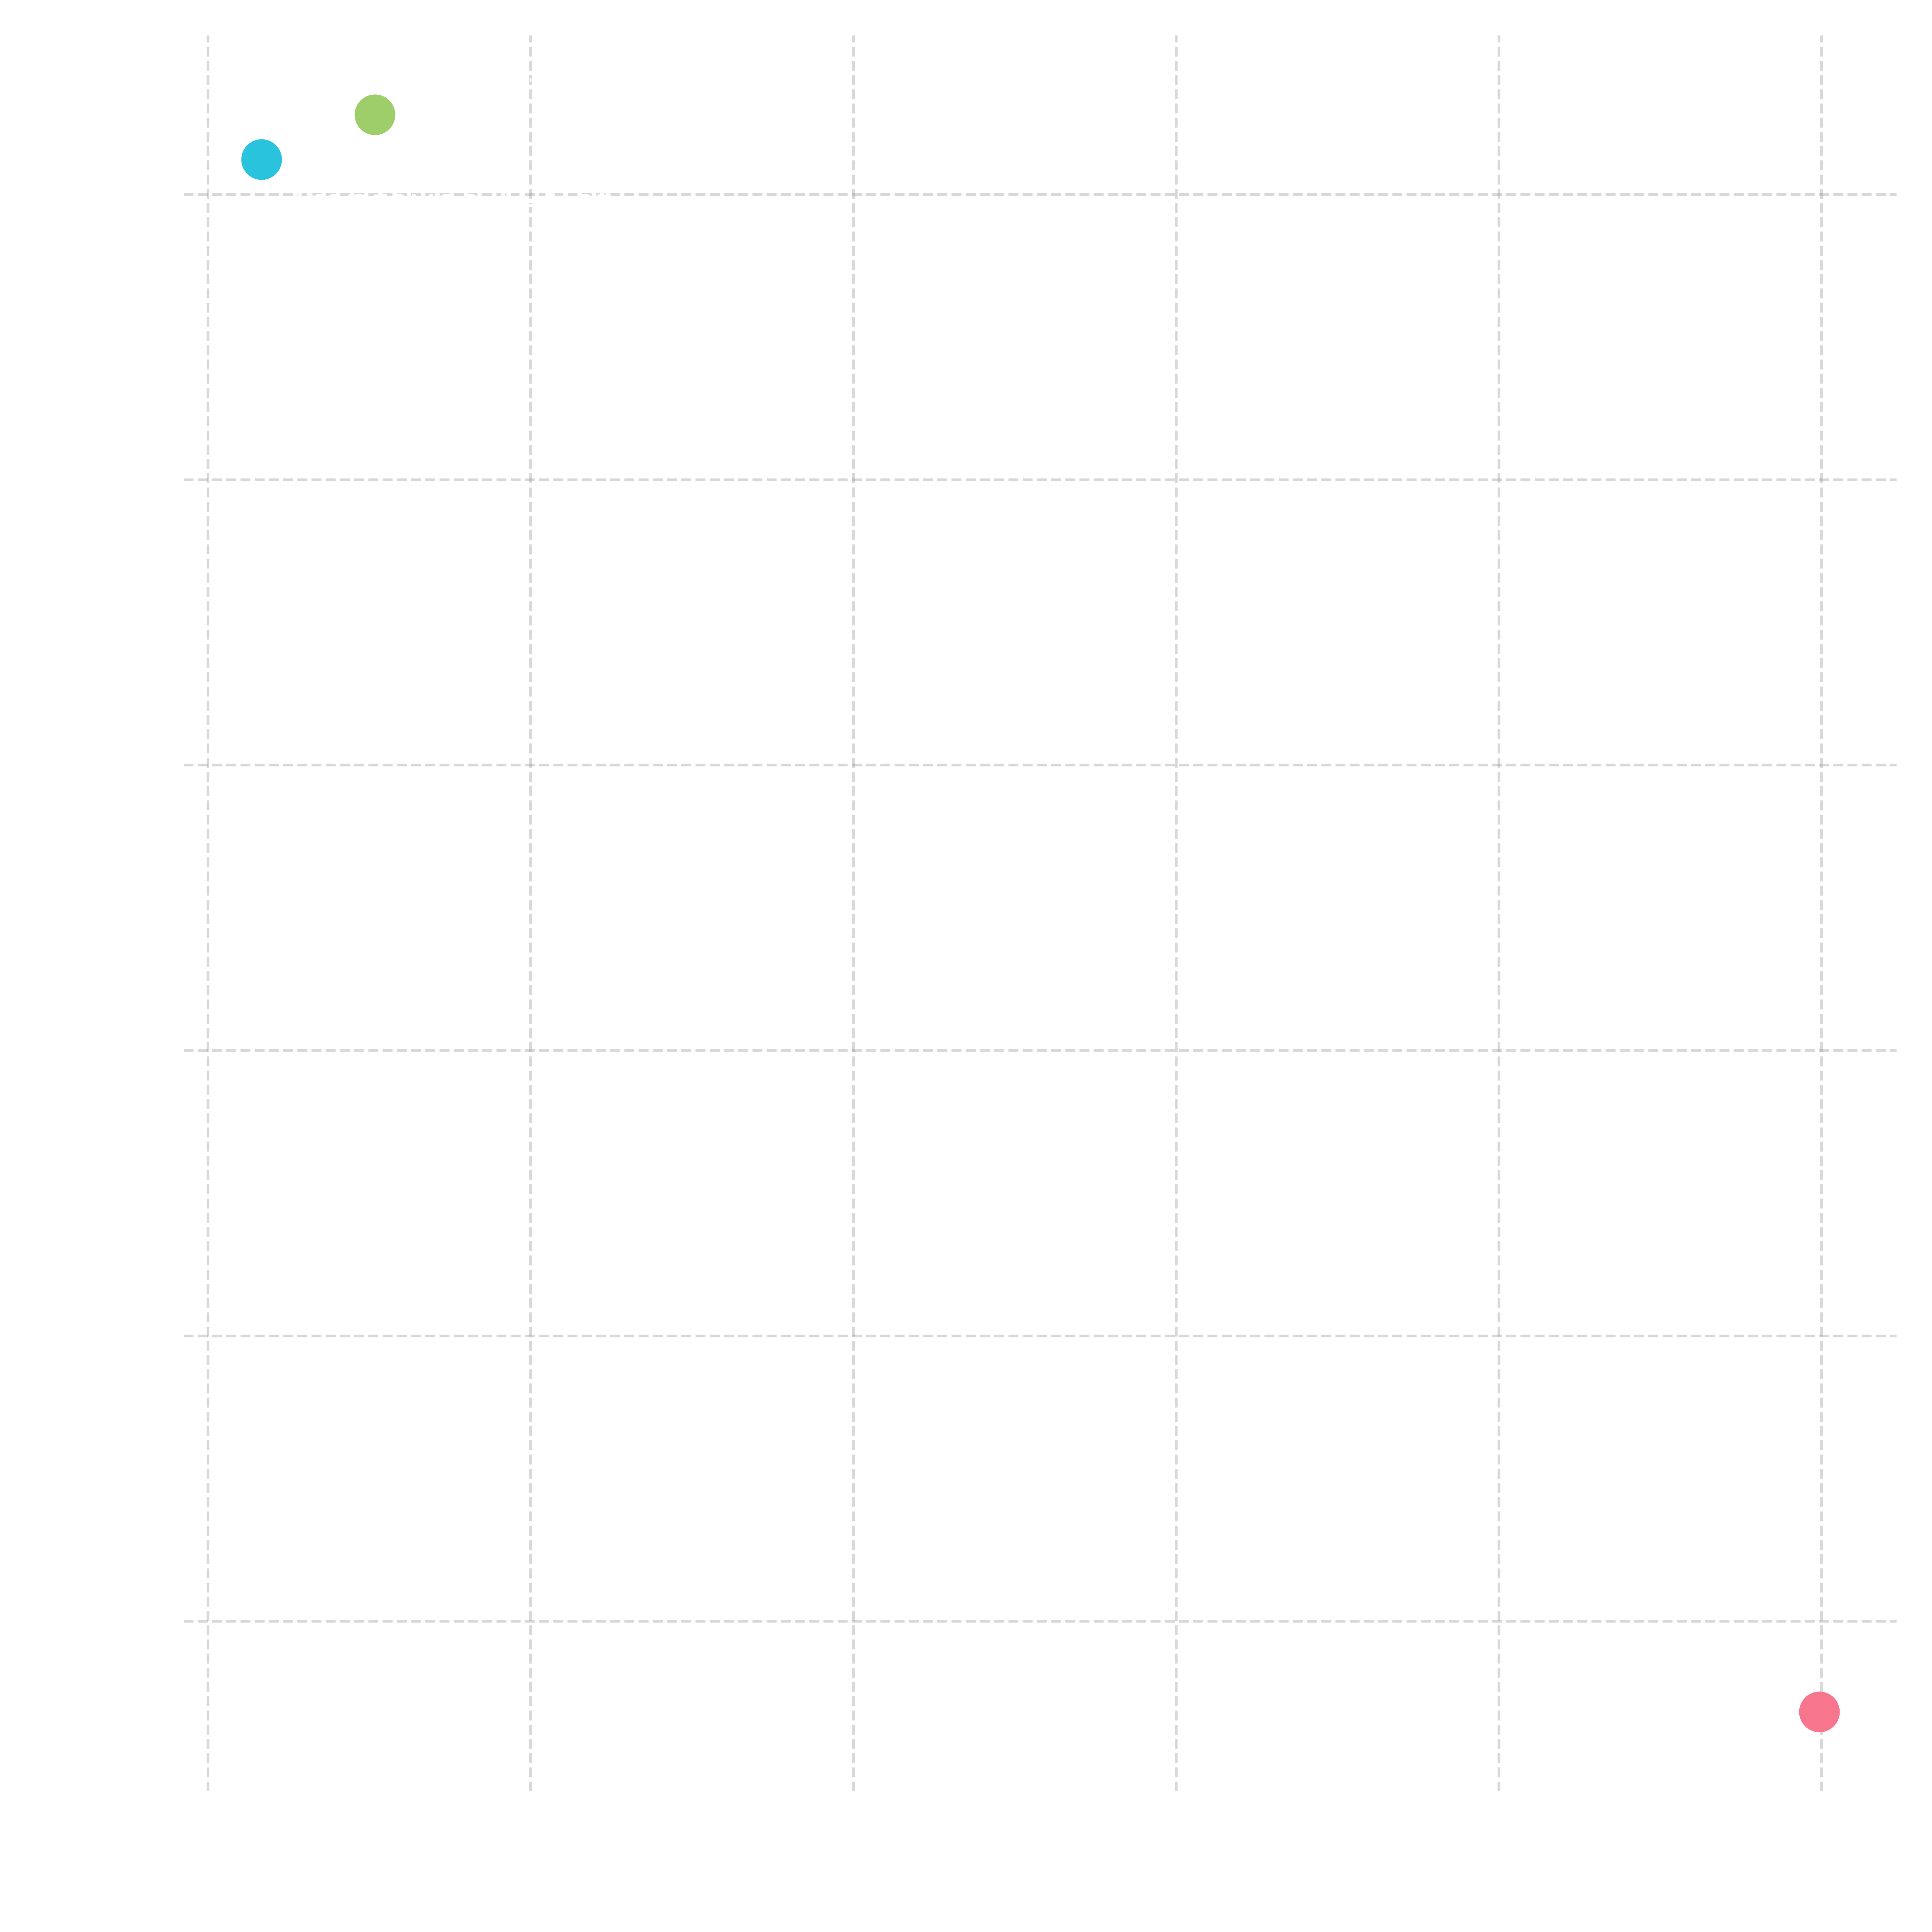
\includegraphics[width=\textwidth]{params_vs_accuracy2.png}
			\end{figure}
		\end{minipage}

\end{frame}

\begin{frame}
    
    \frametitle{Conclusion}

    Possible improvements:
    \vspace{0.2cm}
    \begin{itemize}
        \item Use original image size for better classification results
        \item Use larger dataset to train the VIT model
        \item Enlarge the VIT model for better performance
        \item Attempt transfer learning with VIT model
        \item Test different architectures for the segmentation task
        \item Fully exploit segmentation dataset
        \item Perform complete hyperparameter search for the segmentation models
        \item Use metadata information to predict patient's survival days
    \end{itemize}

\end{frame}

\section{References}

% \begin{frame}

%     [1] B. H. Menze et al. "The Multimodal Brain Tumor Image Segmentation Benchmark (BRATS)", IEEE Transactions on Medical Imaging 34(10), 1993-2024 (2015) DOI: 10.1109/TMI.2014.2377694

%     [2] S. Bakas et al. "Advancing The Cancer Genome Atlas glioma MRI collections with expert segmentation labels and radiomic features", Nature Scientific Data, 4:170117 (2017) DOI: 10.1038/sdata.2017.117

%     [3] S. Bakas et al. "Identifying the Best Machine Learning Algorithms for Brain Tumor Segmentation, Progression Assessment, and Overall Survival Prediction in the BRATS Challenge", arXiv preprint arXiv:1811.02629 (2018)

%     [4] S. Bakas et al. "Segmentation Labels and Radiomic Features for the Pre-operative Scans of the TCGA-GBM collection", The Cancer Imaging Archive, 2017 DOI: 10.7937/K9/TCIA.2017.KLXWJJ1Q

%     [5] S. Bakas et al. "Segmentation Labels and Radiomic Features for the Pre-operative Scans of the TCGA-LGG collection", The Cancer Imaging Archive, 2017 DOI: 10.7937/K9/TCIA.2017.GJQ7R0EF

%     [6] Alex Krizhevsky et al. "ImageNet classification with deep convolutional neural networks", Commun. ACM 60, 6 (June 2017), 84–90, https://doi.org/10.1145/3065386

% \end{frame}
% \begin{frame}

%     [7] A. Dosovitskiy et al. "An Image is Worth 16x16 Words: Transformers for Image Recognition at Scale", International Conference on Learning Representations http://openreview.net/forum?id=YicbFdNTTy

%     [8] Omer, A.A.M. "Image Classification Based on Vision Transformer", Journal of Computer and Communications, 12, 49-59 (2024) https://doi.org/10.4236/jcc.2024.124005

%     [9] Ronneberger, O., Fischer, P., \& Brox, T. "U-Net: Convolutional Networks for Biomedical Image Segmentation", In Nassir Navab, Joachim Hornegger, William M. Wells, \& Alejandro F. Frangi (Eds.), Medical Image Computing and Computer-Assisted Intervention -- MICCAI 2015, 234–241 https://doi.org/10.1007/978-3-319-24574-4_28

%     [10] Chollet, F. "Xception: Deep Learning with Depthwise Separable Convolutions", CoRR, abs/1610.02357 http://arxiv.org/abs/1610.02357

%     [11] Liu, Z., Mao, H., Wu, C.-Y., Feichtenhofer, C., Darrell, T., \& Xie, S. "A ConvNet for the 2020s", arXiv preprint arXiv:2201.03545 https://arxiv.org/abs/2201.03545

%     [12] Sandler, M. et al. "Inverted Residuals and Linear Bottlenecks: Mobile Networks for Classification, Detection and Segmentation", CoRR, abs/1801.04381 http://arxiv.org/abs/1801.04381

%     [13] Oktay, O. et al. "Attention U-Net: Learning Where to Look for the Pancreas", CoRR, abs/1804.03999 http://arxiv.org/abs/1804.03999

% \end{frame}

\begin{frame}

    \frametitle{References}

	{\fontsize{8pt}{7.2}\selectfont

    [1] B. H. Menze et al. ``The Multimodal Brain Tumor Image Segmentation Benchmark (BRATS)'', IEEE Transactions on Medical Imaging 34(10), 1993-2024 (2015) DOI: 10.1109/TMI.2014.2377694\\
	\vspace{1em}

    [2] S. Bakas et al. ``Advancing The Cancer Genome Atlas glioma MRI collections with expert segmentation labels and radiomic features'', Nature Scientific Data, 4:170117 (2017) DOI: 10.1038/sdata.2017.117\\
	\vspace{1em}

    [3] S. Bakas et al. ``Identifying the Best Machine Learning Algorithms for Brain Tumor Segmentation, Progression Assessment, and Overall Survival Prediction in the BRATS Challenge'', arXiv preprint arXiv:1811.02629 (2018)\\
	\vspace{1em}

    [4] S. Bakas et al. ``Segmentation Labels and Radiomic Features for the Pre-operative Scans of the TCGA-GBM collection'', The Cancer Imaging Archive, 2017 DOI: 10.7937/K9/TCIA.2017.KLXWJJ1Q\\
	\vspace{1em}

    [5] S. Bakas et al. ``Segmentation Labels and Radiomic Features for the Pre-operative Scans of the TCGA-LGG collection'', The Cancer Imaging Archive, 2017 DOI: 10.7937/K9/TCIA.2017.GJQ7R0EF\\
	\vspace{1em}

    [6] Alex Krizhevsky et al. ``ImageNet classification with deep convolutional neural networks'', Commun. ACM 60, 6 (June 2017), 84--90, \azure{\url{https://doi.org/10.1145/3065386}}\\
	}

\end{frame}
\begin{frame}

    \frametitle{References}

	{\fontsize{8pt}{7.2}\selectfont

    [7] A. Dosovitskiy et al. ``An Image is Worth 16x16 Words: Transformers for Image Recognition at Scale'', International Conference on Learning Representations \azure{\url{http://openreview.net/forum?id=YicbFdNTTy}}\\
	\vspace{0.7em}

    [8] Omer, A.A.M. ``Image Classification Based on Vision Transformer'', Journal of Computer and Communications, 12, 49-59 (2024) \azure{\url{https://doi.org/10.4236/jcc.2024.124005}}\\
	\vspace{0.7em}

    [9] Ronneberger, O., Fischer, P., \& Brox, T. ``U-Net: Convolutional Networks for Biomedical Image Segmentation'', In Nassir Navab, Joachim Hornegger, William M. Wells, \& Alejandro F. Frangi (Eds.), Medical Image Computing and Computer-Assisted Intervention -- MICCAI 2015, 234--241 \azure{\url{https://doi.org/10.1007/978-3-319-24574-4_28}}\\
	\vspace{0.7em}

    [10] Chollet, F. ``Xception: Deep Learning with Depthwise Separable Convolutions'', CoRR, abs/1610.02357 \azure{\url{http://arxiv.org/abs/1610.02357}}\\
	\vspace{0.7em}

	[11] Liu, Z., Mao, H., Wu, C.-Y., Feichtenhofer, C., Darrell, T., \& Xie, S. ``A ConvNet for the 2020s'', arXiv preprint arXiv:2201.03545 \azure{\url{https://arxiv.org/abs/2201.03545}}\\
	\vspace{0.7em}

	[12] Sandler, M. et al. ``Inverted Residuals and Linear Bottlenecks: Mobile Networks for Classification, Detection and Segmentation'', CoRR, abs/1801.04381 \azure{\url{http://arxiv.org/abs/1801.04381}}\\
	\vspace{0.7em}

	[13] Oktay, O. et al. ``Attention U-Net: Learning Where to Look for the Pancreas'', CoRR, abs/1804.03999 \azure{\url{http://arxiv.org/abs/1804.03999}}\\

	}

\end{frame}

\end{document}
